\chapter{Resultados y análisis\label{sec:resultados}}
En este capítulo se detallan las medidas para la comprobación del sensor de ultrasonido. Para ello, se han realizado primero medidas en estático que han permitido la comprobación de la conectividad del sensor con el PC y a continuación se han realizado en dinámico para comprobar que es viable la medida de separación entre piernas para poder después medir la distancia de separación entre pasos.

\section{Resultados}

\subsection{Medidas en estático}

Mediante el set-up de medida representado en anteriores apartados se realizan pruebas en estático del sensor de ultrasonidos para verificar que funciona correctamente. Para ello, se realizaron medidas a una distancia de 5 cm, de 35 cm y de 60 cm. No se consideraron distancias mayores ya que creemos que la separación entre piernas no superará ese rango de distancias.

\begin{itemize}
	\item \textbf{Medida de 5 cm}
	
	En la Figura \ref{fig:ultra5} aparece representada la medida para una distancia de 5 cm. 
	
	\begin{figure}[H]
		\centering
		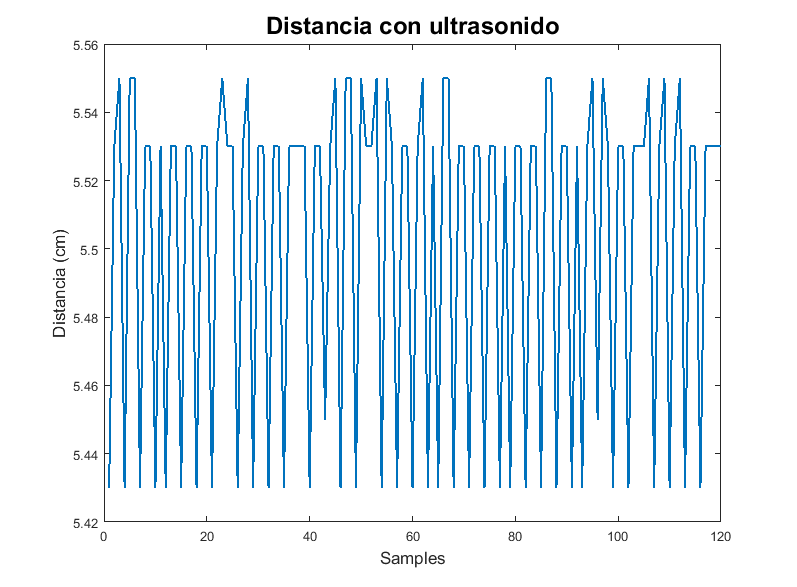
\includegraphics[width=17 cm,height=11 cm]{./graphics/5}
		\caption{Medida de sensor de ultrasonido en estático.} \label{fig:ultra5}
		
	\end{figure}
	\item \textbf{Medida de 35 cm}
	
	En la Figura \ref{fig:ultra} se representa una medida con un obstáculo situado a 35 cm del sensor. 
	
	\begin{figure}[H]
		\centering
		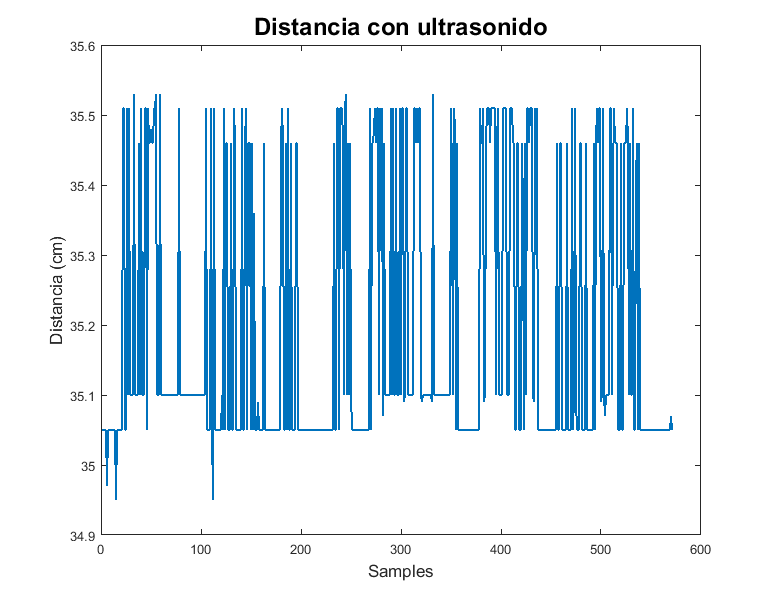
\includegraphics[width=16 cm,height=8.5 cm]{./graphics/aa}
		\caption{Medida de sensor de ultrasonido en estático.} \label{fig:ultra}
		
	\end{figure}
	
	\item \textbf{Medida de 60 cm}
	
	En la Figura \ref{fig:ultra60} se representa la medida realizada a 60 cm. 
	\begin{figure}[H]
		\centering
		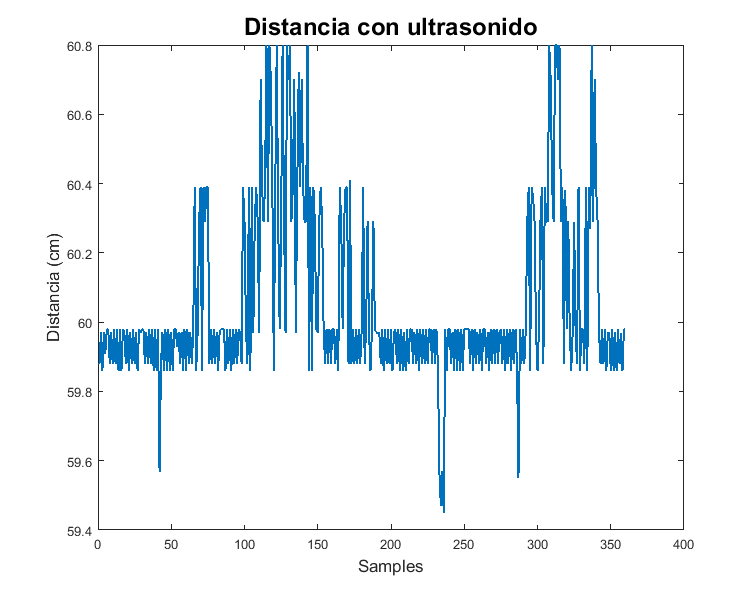
\includegraphics[width=16 cm,height=8 cm]{./graphics/60}
		\caption{Medida de sensor de ultrasonido en estático.} \label{fig:ultra60}
		
	\end{figure}
	
\end{itemize}

Para estimar la precisión del sistema se han calculado tanto errores absolutos como relativos de cada una de las medidas.


\subsection{Medidas en dinámico}

En la Figura \ref{fig:ultrasonido_corto} se observa cómo la distancia es de 28,38 cm. Dicho resultado se ha obtenido cuando la persona a la que se media daba un paso.

\begin{figure}[H]
	\centering
	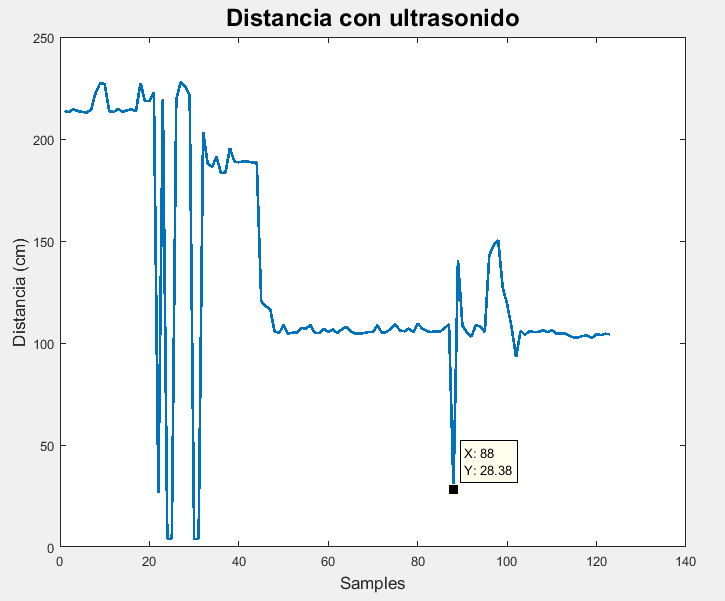
\includegraphics[width=16 cm,height=8 cm]{./graphics/ultrasonido_corto}
	\caption{Medida sensor de ultrasonido en dinámico} \label{fig:ultrasonido_corto}
	
\end{figure}

En la Figura \ref{fig:ultrasonido_corto2} se representa otra medida realizada por diferente sujeto y dando un paso de diferente longitud. En este caso también la distancia entre las piernas es de 24,55 cm

\begin{figure}[H]
	\centering
	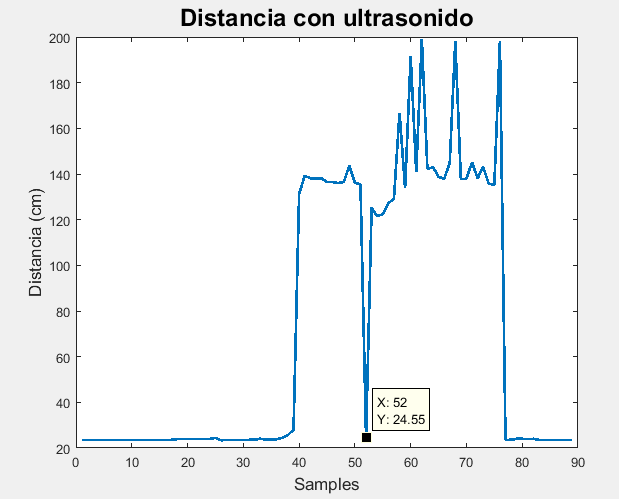
\includegraphics[width=16 cm,height=9 cm]{./graphics/dinam2}
	\caption{Medida sensor de ultrasonido en dinámico} \label{fig:ultrasonido_corto2}
	
\end{figure}

Con los datos de distancia calculados mediante los diferentes sensores se puede calcular la distancia de separación entre pasos mediante lo detallado en el Capítulo \ref{sec:disenho}.


\section{Análisis de resultados}

En la Tabla \ref{tabla:medidas 43 cm} aparecen representados los datos obtenidos en las medidas con el sensor en estático. Se observa como la precisión es mayor en valores intermedios de distancia, es decir en aquellos valores en los que estará comprendido el valor de distancia de separación entre piernas. El mayor error se da para el caso de 5 cm pero en este contexto la distancia que se desea medir será mayor a ese valor.


\begin{table}[H]
	\centering
	\begin{tabular}[t]{|c|c|c|c| }
		\hline
		& Medida 1 (5 cm) & Medida 2 (35 cm) & Medida 3 (60 cm) \\
		\hline
		Medida  & 5 cm   & 35 cm  & 60 cm  \\
		\hline
		Error absoluto  & 0.5022 cm &  0.1870 cm  &  0.1906 cm \\ 
		\hline
		Error relativo  & 10,0433\% &  0.5342\%  &  0.2816\% \\ 
		\hline
	\end{tabular}
	\caption{Tabla medidas en estático}
	\label{tabla:medidas 43 cm}
\end{table}

En la Tabla \ref{tabla:medidas 80 cm} se representan cinco medidas realizadas a diferentes sujetos con el sensor mientras se efectúa un paso.

\begin{table}[H]
	\centering
	\begin{tabular}[t]{|c|c|c|c|c|}
		\hline
		Medida 1 & Medida 2 & Medida 3 & Medida 4 & Medida 5\\
		\hline
		28,38 cm & 24,55 cm & 23,42 cm & 24,89 cm & 26,55 cm \\
		\hline
		
	\end{tabular}
	\caption{Tabla medidas en dinámico}
	\label{tabla:medidas 80 cm}
\end{table}

Para determinar la validez y fiabilidad de los medidas realizadas en dinámico se pidió a los sujetos que participaron en la validación que realizarán pasos sobre marcas en el suelo, situadas a distancias fijas. Estas marcas simulan diferentes longitudes de paso (Figura \ref{fig:marcas}). D1 es de aproximadamente 25 cm pero dependiendo del sujeto puede variar.

\begin{figure}[H]
	\centering
	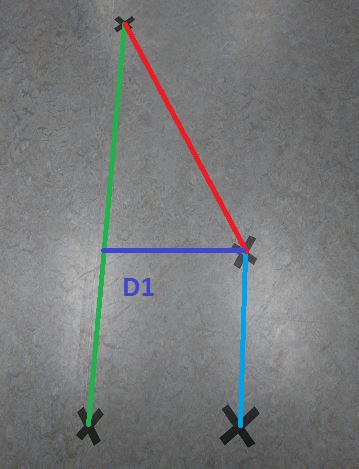
\includegraphics[width=10 cm,height=11 cm]{./graphics/marcas}
	\caption{Validación del sensor de ultrasonidos en dinámico} \label{fig:marcas}
	
\end{figure}

